% SIAM Article Template
\documentclass[review,hidelinks,onefignum,onetabnum]{siamart220329}
\usepackage{mathtools}
\usepackage{tikz}
\usepackage{algorithmic}
\Crefname{ALC@unique}{Line}{Lines}

\let\vec\mathbf
\DeclarePairedDelimiter\norm{\lVert}{\rVert}
% Information that is shared between the article and the supplement
% (title and author information, macros, packages, etc.) goes into
% ex_shared.tex. If there is no supplement, this file can be included
% directly.

% SIAM Shared Information Template
% This is information that is shared between the main document and any
% supplement. If no supplement is required, then this information can
% be included directly in the main document.


% Packages and macros go here
\usepackage{lipsum}
\usepackage{amsfonts}
\usepackage{graphicx}
\usepackage{epstopdf}
\usepackage{algorithmic}
\ifpdf
  \DeclareGraphicsExtensions{.eps,.pdf,.png,.jpg}
\else
  \DeclareGraphicsExtensions{.eps}
\fi

% Add a serial/Oxford comma by default.
\newcommand{\creflastconjunction}{, and~}

% Used for creating new theorem and remark environments
\newsiamremark{remark}{Remark}
\newsiamremark{hypothesis}{Hypothesis}
\crefname{hypothesis}{Hypothesis}{Hypotheses}
\newsiamthm{claim}{Claim}

% Sets running headers as well as PDF title and authors
\headers{The lightening Virtual Element Method''}{M. L. Trezzi, and U. Zerbinati}

% Title. If the supplement option is on, then "Supplementary Material"
% is automatically inserted before the title.
\title{When rational function meets virtual elements:\\``The lightning Virtual Element Method''\thanks{Submitted to the editors DATE.
\funding{This work was funded by the Fog Research Institute under contract no.~FRI-454.}}}

% Authors: full names plus addresses.
\author{M. L. Trezzi\thanks{Università di Pavia, Pavia, Italia 
  (\email{ddoe@imag.com}).}
\and U. Zerbinati\thanks{Univeristy of Oxford, Oxford, United Kingdom
  (\email{umberto.zerbinati@maths.ox.ac.uk})}
}

\usepackage{amsopn}
\DeclareMathOperator{\diag}{diag}


%%% Local Variables: 
%%% mode:latex
%%% TeX-master: "ex_article"
%%% End: 


% Optional PDF information
\ifpdf
\hypersetup{
  pdftitle={When rational function meet virtual elements: ``The lightning Virtual Element Method''},
  pdfauthor={M. L. Tezzi, and U. Zerbinati}
}
\fi

% The next statement enables references to information in the
% supplement. See the xr-hyperref package for details.

\externaldocument[][nocite]{ex_supplement}

% FundRef data to be entered by SIAM
%<funding-group specific-use="FundRef">
%<award-group>
%<funding-source>
%<named-content content-type="funder-name"> 
%</named-content> 
%<named-content content-type="funder-identifier"> 
%</named-content>
%</funding-source>
%<award-id> </award-id>
%</award-group>
%</funding-group>

\begin{document}

\maketitle

% REQUIRED
\begin{abstract}
Since its introduction the Virtual Element Method (VEM) has been recognised by the numerical analysis community as a valuable tool for the solution of partial differential equations (PDEs).
The mathematical infrastructure is what makes the VEM shine and reveals all its advantages, the (not so) downsides of the VEM are the practical aspects of its implementation.
The true brilliance behind the VEM is the use of the so-called projection operators that allow you to assemble the stiffness and mass matrices without the necessity of actually computing the virtual component of the basis functions.
Following the ``no free lunch'' principle resorting to projection operators for assembling local matrices results in a lack of coercivity that requires the use of an additional stabilisation term in the weak formulation of the problem.
The lightning Virtual Element Method here proposed aims to get rid of the stabilisation term by actually computing, in an extremely efficient manner, the virtual component of the local VEM basis functions.
In particular, the lightning VEM approximates the virtual part of the basis functions using rational functions with poles clustered exponentially close to the corners of each element of the polynomial tessellation.
This results in two great advantages, first the mathematical analysis of a priori error estimates is much easier and essentially identical to the one for any other non-conforming Galerkin discretisation.
Furthermore, the fact that the lightning VEM truly computes the basis functions allows the user to access the pointwise value of the numerical solution without needing any reconstruction techniques.
The cost of the local construction of the VEM basis is the implementation price that one has to pay for the advantages of the lightning VEM method, but as we will see the embarrassingly parallelizable nature of this operation will ultimately result in a cost-efficient scheme compared to standard VEM and FEM.
\end{abstract}

% REQUIRED
\begin{keywords}
example, \LaTeX
\end{keywords}

% REQUIRED
\begin{MSCcodes}
68Q25, 68R10, 68U05
\end{MSCcodes}

\section{Introduction}
Since its introduction in \cite{VEMBasic} the Virtual Element Method (VEM) has been recognised by the numerical analysis community as a valuable tool for the solution of partial differential equations (PDEs).
One of the key advantages of the VEM is that it allows any type of polygonal meshes, thanks to the introduction of a virtual component in the local basis functions.
We will discuss this aspect in greater detail in a later section.
Non-polygonal meshes can also be used more naturally than in iso-parametric finite elements, \cite{CurvedVEM},
Furthermore, given the rise of structure-preserving discretisation it is worth mentioning the VEM allows to mimic many interesting physical structures that arise at the level of the continuous PDE, \cite{VEMStokes}.
One improvement in this realm is that the VEM contrary to the standard finite element method (FEM) can be used to construct arbitrary low-order structure-preserving discretisation.
The sophisticated mathematical infrastructure that allows proving accurate a priori error estimates, which are a key advantage of the FEM, can also be applied with very few adjustments also to the VEM.
Another feature of the VEM, perhaps the one that the authors of this paper consider of the greatest importance, is the ability to easily produce discretisation with a high order of continuity, a property that is well known to be a weak spot of classical FEM.
It is also worth mentioning that VEM accuracy can be improved with the $p$ and $hp$ versions of VEM introduced in \cite{hpVEM}, clearly this is a direct consequence of the intimate relation between the FEM and VEM.
The advantages previously mentioned lead to the application of the VEM to a wide variety of problems going from linear elasticity \cite{LavadinaEl},\cite{BMEl},\cite{LovadinaEl2}; fluid-dynamics \cite{Inc1},\cite{Inc2},\cite{Inc3}; fourth-order problems \cite{F1},\cite{F2},\cite{F3}; acoustic wave propagation and Helmholtz problem \cite{Wave1},\cite{Perugia}; magnetostatics \cite{M1},\cite{M2}.
While the mathematical infrastructure is what makes the VEM shine and reveals all the advantages listed above the (not so) dark sides of the VEM are the practical aspects of its implementation.
The true brilliance behind the VEM is the use of the so-called projection operators that allow assembling stiffness and mass matrices without the necessity of really computing the virtual component of the basis functions.
Following the ``no free lunch'' principle resorting to projection operators to assemble local matrices result in a lack of coercivity that require the use of an additional stabilisation term in the weak formulation of the problem.
The lightning Virtual Element Method here proposed aims to get rid of the stabilisation term by actually computing, in an extremely efficient manner, the virtual component of the local VEM basis functions.
In particular, the lightning VEM approximates the virtual part of the basis functions using rational functions with poles clustered exponentially close to the corners of each element of the polynomial tessellation.
It is worth mentioning that in the literature other ideas have been proposed in order to get rid of the stabilisation term, we redirect the interested reader to \cite{BerroneE2VEM,BerroneE2VEM2,E2VEMEig,AdaptiveE2VEM}.
The key difference between the lightning VEM and the method previously mentioned is the fact that the lightning VEM doesn't make use of any projection operators.
This results in two great advantages, first the mathematical analysis of a priori error estimates is much easier and essentially identical to the one for any other non-conforming Galerkin discretisation.
Furthermore, the fact that the lightning VEM truly computes the basis function allows the user to access pointwise value of the numerical solution without the need for any reconstruction technique.
One common reconstruction technique is based on polynomial interpolation and might require the triangulation of the polygonal mesh we considered at the beginning.
It is important to mention that one key aspect of many implementations of the FEM is the use of affine transformations to standardise the assembly of mass, transport and stiffness matrices as a finite element routine operating on a reference element.
Such a construction has worked well for standard finite element discretisation but more complicated elements such as the Argyris and Bell triangles require a more complicated mapping. For this reason, modern finite element solvers might resort to a more general transformation, such as the one described in \cite{Kirby}.
Another library such as MODULEF, resorts to the local construction of basis functions on each element.
The local construction of VEM basis is the implementation price that one has to pay for the advantages of the lighenting VEM method, but as we will see the embarrassingly parallelizable nature of this operation will ultimately result in a cost-efficient scheme compared to standard VEM and FEM.
\section{The virtual element space}
Let us consider two Hilbert spaces $X,Y$ and a differential operator $Q$ that is linear and bounded.
Given an element $f\in Y$ we consider the linear partial differential equation
\begin{equation}
  \textrm{find } u\in X\textrm{ such that }Q u = f,\textrm{ with }f\in Y.\label{eq:strong}
\end{equation}
We further assume that the above operator equation can be recast in the form of a variational equation, i.e. let $V$ be a Hilbert space, $f\in V^*$ and $\mathcal{Q}:V\times V\to \mathbb{R}$ a continuous and coercive bilinear form then we consider the problem
\begin{equation}
  \textrm{find }u\in V\textrm{ such that }\mathcal{Q}(u,v)=\;<\!\!f,v\!\!>\textrm{ for any }v\in V.\label{eq:var}
\end{equation} 
In particular, we will say that \eqref{eq:var} is the variational equation corresponding to \eqref{eq:strong} if $u$ solving \eqref{eq:strong} also solves \eqref{eq:var} and if it exists $u\in X$ that solves \eqref{eq:var} it is also a solution of \eqref{eq:strong}.
With the hypothesis that the bilinear form $\mathcal{Q}(\cdot,\cdot)$ is coercive and continuous, the well-posedness of the variational problem comes from Lax-Milgram lemma, \cite{Evans}.
\begin{remark}
  The typical example of the above type of partial differential equation is the transport-diffusion equation, i.e.
  \begin{align}
      \Delta u + \gamma u = f \;\;&in\; \Omega,\label{eq:transportDiffusion}\\
      u\equiv 0 \;\;& on\;\partial\Omega.\nonumber
  \end{align}
  In particular we will assume $f\in \mathcal{L}^2(\Omega)$ and $u\in H^2(\Omega)$, where $\Omega\subset\mathbb{R}^2$ is a pre-compact domain with smooth boundary.
  The variational equation corresponding to \eqref{eq:transportDiffusion} is the following
  \begin{equation}
    \textrm{find } u\in H^1_0(\Omega) \textrm{ s.t. } \int_{\Omega}\!\nabla u\cdot \nabla v\,d\vec{x} + \gamma\!\int_{\Omega}\!uv \,d\vec{x}= \int_{\Omega}\!fv\,d\vec{x}, \textrm{ for any }v\in H^1_0(\Omega).\label{eq:weakTransportDiffusion}
  \end{equation}
\end{remark}
We consider now a conforming Galerkin approximation of \eqref{eq:var}, i.e. we fix a discrete space $V_h\subset V$ and consider the variational problem
\begin{equation}
  \textrm{find }u_h\in V_h\textrm{ such that }\mathcal{Q}(u_h,v_h)=\;<\!\!f,v_h\!\!>\textrm{ for any }v_h\in V_h.\label{eq:varDiscrete}
\end{equation} 
Notice that once again the well-posedness of the variational problem comes from Lax-Milgram lemma thanks to the continuity and coercivity of the bilinear form $\mathcal{Q}(\cdot,\cdot)$ together with the fact that $V^*\subset V_h^*$.
As it appears obvious one of the key ingredients of any conforming Galerkin scheme is the way $V_h$ is constructed.
In the context of the virtual element method, we assume that $\Omega$ is a polygonal domain and start by considering any polygonal mesh $\mathcal{T}_h$.
We then proceed to construct a local discrete space, i.e. for any $K\in \mathcal{T}_h$ we denote $e$ the edges of $K$ and construct the local VEM space as
\begin{equation}
  V_h^k(K) = \Big\{u \in C^2(K)\;:\; u_{|e} \in \mathbb{P}_{k}(e)\; and \; \mathcal{L} u \in \mathbb{P}_{k-2}(K)\Big\},\label{eq:localVEM}
\end{equation}
where we have denoted $\mathbb{P}_k(\cdot)$ the space of polynomials of order $k$, and we have adopted the usual convention $\mathbb{P}_{-1} = \{0\}$. Once the local VEM space has been constructed we proceed defining the space $V_h$ as 
\begin{equation}
  V_h = \Big \{u \in H^1_0(\Omega)\;:\; u \in V_h^k(K) \; \forall K \in \mathcal{T}_h\Big \}.
\end{equation} 
The operator $\mathcal{L}$ has been left ambiguous by choice, since for the well-posedness of \eqref{eq:localVEM} any elliptic partial differential operator would do the job.
To retrieve optimal approximation property it will be convenient also to assume that $\mathbb{P}_{k}$ is a subset of the co-domain of the operator $\mathcal{L}$ when applied to the space $\mathbb{P}_{k-2}$ with the constraint of having boundary data in $\mathbb{P}_k$.
A common misunderstanding when first approaching the VEM is to think in terms of Treftz methods, i.e. assume that the operator $\mathcal{L}$ has to be the same as $Q$. This is not the case we should think of $\mathcal{L}$ only in terms of the conformity we are interested in.
\begin{remark}
  If we desire an $H^1$ conforming discretisation the most common choice of operator $\mathcal{L}$ is the negative Laplacian.

  Once again we can use the Lax-Milgram lemma to prove the well-posedness of \eqref{eq:localVEM} since $-\Delta$ is an elliptic operator.
\end{remark}
\begin{remark}
  In general, if we require an $H^k$ conforming discretisation the most common choice of $\mathcal{L}$ would be the polylaplacian, in particular we will consider $-\Delta^k$.
  Of course, we need to modify slightly our definition of local VEM space to accommodate for the fact that we have to prescribe not only the value of the solution at the boudnary but also of the first $k-1$ normal derivatives.
  More detail on this topic can be found in \cite{F1,F2,F3,Polylapcian,PolyLaplacianPt2}.
\end{remark}
At this point, the theory of VEM and the lightning VEM method diverge slightly. The idea behind the virtual element method is to consider a slightly different variational problem than \eqref{eq:varDiscrete}, paying the price of a non-coercive bilinear form.
\begin{figure}[h]
	\centering
	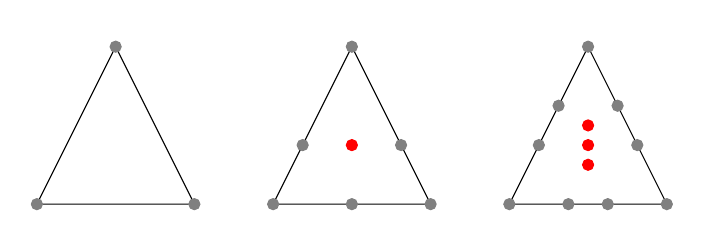
\begin{tikzpicture}[scale=0.5]
	\draw (-2,0) node[anchor=north]{$$}
	-- (2,0) node[anchor=north]{$$}
	-- (0,4) node[anchor=south]{$$}
	-- cycle;
	\filldraw [gray] (-2,0) circle (4pt);
	\filldraw [gray] (0,4) circle (4pt);
	\filldraw [gray] (2,0) circle (4pt);
	
	\draw (4,0) node[anchor=north]{$$}
	-- (6,4) node[anchor=north]{$$}
	-- (8,0) node[anchor=south]{$$}
	-- cycle;
	\filldraw [gray] (4,0) circle (4pt);
	\filldraw [gray] (6,4) circle (4pt);
	\filldraw [red] (6,1.5) circle (4pt);
	\filldraw [gray] (8,0) circle (4pt);
	\filldraw [gray] (6,0) circle (4pt);
	\filldraw [gray] (4.75,1.5) circle (4pt);
	\filldraw [gray] (7.25,1.5) circle (4pt);
	
	\draw (10,0) node[anchor=north]{$ $} -- (12,4) node[anchor=north]{$ $} -- (14,0) node[anchor=south]{$ $} -- cycle;
	\filldraw [gray] (10,0) circle (4pt);
	\filldraw [gray] (12,4) circle (4pt);
	\filldraw [gray] (14,0) circle (4pt);
	\filldraw [red] (12,2) circle (4pt);
	\filldraw [red] (12,1.5) circle (4pt);
	\filldraw [red] (12,1) circle (4pt);
	\filldraw [gray] (11.5,0) circle (4pt);
	\filldraw [gray] (12.5,0) circle (4pt);
	\filldraw [gray] (10.75,1.5) circle (4pt);
	\filldraw [gray] (13.25,1.5) circle (4pt);
	\filldraw [gray] (11.25,2.5) circle (4pt);
	\filldraw [gray] (12.75,2.5) circle (4pt);
	\end{tikzpicture}
	\caption{From left to right we observe the degrees of freedom of $k=1,2,3$ for virtual element methods.}
	\label{fig:VEMDofs}
\end{figure}
\section{The lightning approximation}
The key idea behind the lightning VEM is to consider a different local discrete space which is obtained approximating $V_h^k(K)$ using rational functions with poles clustered exponentially close to the corners of $K$.
For the sake of clarity, we will focus our discussion on the lowest order case, $k=1$, and choose $\mathcal{L}=-\nabla$. We will discuss in a later section how to deal with the case $k>1$ and the case where higher conformity is required.
Thanks to the linearity of the Laplacian if $K$ has $N_k$ edges to construct $V_h^k(K)$ we are interested in solving $N_K(k+1)$ problems of the form
\begin{align}
    \Delta u_i^{(e)} = 0 \;\;&in\; \Omega,\label{eq:basisProblem}\\
    u_i^{(e)} = \varphi_i^{(e)} \;\; & on\;\partial\Omega.\nonumber
\end{align}
Ideally, if we are structured rectangular mesh we know how to solve this problem exactly.
As the geometry of $K$ gets more complicated we need to find an efficient way of solving \eqref{eq:basisProblem}.
To slay this dragon we turn to the lightning Laplace solver presented in \cite{LighteningLaplace,LighteningLaplace2}.
The idea behind the lightning Laplace method is to search for an approximation $\hat{u}_i^{(e)}$ of $u_i^{(e)}$ of the form,
\begin{equation}
	\hat{u}_i^{(e)} = \Re\bigg\{\sum_{j=0}^{N_P}\frac{a_j}{z-z_j}+\sum_{j=0}^{N_Z}b_j(z-z_*)^j\bigg\}. 
\end{equation} 
where $\{z_j\}_{j=1}^{N_P}$ and $z_*$ are points in the complex plane.
Finding the optimal coefficients to minimize $\norm{\hat{u}_i^{(e)}-u_i^{(e)}}_{\mathcal{L}^\infty(K)}$ in general is a highly non-linear problem.
To transform this non-linear problem into a linear one the position of the points $\{z_j\}_{j=1}^{N_P}$ and $z_*$ are fixed only based upon the geometry of $K$.
In particular, the $N_P$ poles are clustered exponentially closer to the corners of the polygon $K$. Under this hypothesis, the following result was proven in \cite{LighteningStokes}:
\begin{lemma}
	Let $K$ be a convex polygon with corners $w_1,\dots,w_{N_K}$ and let $f$ be an analytic function on $K$ that is analytic on the interior of each side segment.
	Furthermore, we assume that $f$ can be analytically continued to a disk near any corner $w_k$ with a slit along the exterior bisector of the corner.
	Lastly, we assume that at each corner $w_k$ the function $f$ satisfies $f(z)-f(w_k)=\mathcal{O}(\norm{z-w_k}^\delta)$ as $z\to w_k$, for some $\delta>0$.
	Under these assumptions, there exists a rational function $r$ of the form
	\begin{equation}
		r = \Re\bigg\{\sum_{j=0}^{N_P}\frac{a_j}{z-z_j}+\sum_{j=0}^{N_Z}b_j(z-z_*)^j\bigg\},
	\end{equation}
	with $N_P$ poles $z_j$ only at points exponentially clustered along the exterior bisectors at the corners, such that the following approximation bound holds:
	\begin{equation}
		\norm{f-r}_{\mathcal{L}^\infty(K)} \leq C_K e^{-C\sqrt{N_P}}.
	\end{equation}
\end{lemma}
The exact algorithm used to compute the solution $\hat{u}_i^{(e)}$ of \eqref{eq:localVEM} is presented in Algorithm \ref{alg:lightningLaplace} and we once again redirect the reader interested in more detail to \cite{LighteningLaplace}.
\begin{algorithm}[h]
\caption{
	We compute the solution $\hat{u}_i^{(e)}$ of \eqref{eq:localVEM}.}
	\label{alg:lightningLaplace}
	\begin{algorithmic}[1]
		\REQUIRE{$n_1,\;n_2,\;\dots$ such that $\sqrt{n_1},\;\sqrt{n_2},\;\dots$ is uniformly spread.}
		\FOR{$n \in \{n_1,n_2,\dots\}$}
			\STATE{Fix $N_P \approx nN_K$ and cluster the pole outside $K$ and exponentially close the corners;}
			\STATE{Fix $z_*$ in the interior of $K$ and fix $N_Z \approx N_K$ elements of the monomial basis;}
			\STATE{Choose $M=6N_P+6N_Z+1$ sample points on the boundary and clustered near the corners;}
			\STATE{Evaluate at the sample points to obtain a matrix $A\in \mathbb{R}^{M\times (2N_P+2N_Z+1)}$ and $\vec{d}\in \mathbb{R}^{M}$;}
			\STATE{Solve the least square problem $A\vec{x} \approx \vec{d}$ for the coefficients $\vec{x}=(\vec{a},\vec{b})$;}
			\IF{$\norm{A\vec{x}-\vec{d}}\leq \varepsilon$}
				\STATE{\textbf{break;}}
			\ENDIF
		\ENDFOR
		\STATE{Construct the function $\hat{u}_i^{(e)}$ using the coefficients $\vec{a}$ and $\vec{b}$;}
		\RETURN{$\hat{u}_i^{(e)}$.}
	\end{algorithmic}
\end{algorithm}
Now we are interested in an a priori error estimate for $\norm{u_i^{(e)}-\hat{u}_i^{(e)}}_{L^2(\Omega)}$.
To achieve this we first observe that since  $\sum_{j=0}^{N_P}\frac{a_j}{z-z_j}+\sum_{j=0}^{N_Z}b_j(z-z_*)^j$, it is analytic in the convex-hull described by the vertex of any polygonal element $K$ of the tessellation $\mathcal{T}_h$ where $z_j$ are the vertices of $K$, then its real part is a harmonic function.
We redirect the reader unfamiliar with this notion to \cite{Gilardi,Ahlfors}.

\section*{Acknowledgments}
We would like to acknowledge the assistance of volunteers in putting
together with this example manuscript and supplement.

\bibliographystyle{siamplain}
\bibliography{references}
\end{document}
